%
%
%		Finding: Template
%		Author: the DR
%
%
\renewcommand{\FindingAuthor}{}
% DO NOT USE \par, \newline or any other line breaking command in FindingName => report will not build
\renewcommand{\FindingName}{DummyApplication Signed with a Debug Certificate}
\renewcommand{\Location}{}
\renewcommand{\Component}{META-INF/CERT.RSA}
\renewcommand{\FoundWith}{KeyStore Explorer}
\renewcommand{\TestMethod}{Manual Analysis}
\renewcommand{\CVSS}{N/A}
\renewcommand{\CVSSvector}{N/A}
\renewcommand{\CWE}{}
% Poor-man's combo boxes:
% High, Medium, Low, Info, TBR (To Be Rated)
\renewcommand{\Criticality}{Info}
% Easy, Average, Hard, TBR (To Be Rated)
\renewcommand{\Exploitability}{Hard}
% Access control, Application Design, Information Disclosure, Outdated Software, Security Configuration
\renewcommand{\Category}{TBR}
% Easy, Average, Difficult, TBR (To Be Rated)
\renewcommand{\Detectability}{TBR}


\ReportFindingHeader{\FindingName}


%-------------------------------------------
%	Details                                |
%-------------------------------------------

\subsection*{Details}

The \texttt{dummyapplication.apk} is signed with a debug certificate.

%-<Details>
%-------------------------------------------
%	Impact                                 |
%-------------------------------------------

\subsection*{Impact}

Debug certificates do not meet security standards of the release certificates. 

%-<Impact>
%-------------------------------------------
%	Repeatability                          |
%-------------------------------------------
\pagebreak
\subsection*{Repeatability}


\begin{figure}[H]
\centering
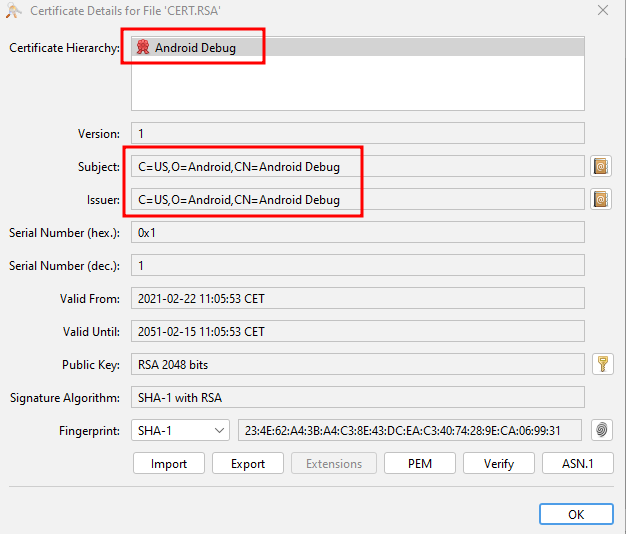
\includegraphics[width=0.7\textwidth,frame]{\CurrentFilePath/DebugCert.png}
\caption{Android debug certificate properties}
\label{figure:DebugCert}
\end{figure}
	

%-<Repeatability>
%-------------------------------------------
%	Countermeasures                        |
%-------------------------------------------

\subsection*{Countermeasures}


%-<Countermeasures>
%-------------------------------------------
%	References - pulls bib entries         |
%-------------------------------------------

\subsection*{References}



%-<References>
